\documentclass[a4paper]{article}

\usepackage{amsmath}
\usepackage{amsfonts}
\usepackage{amssymb}
\usepackage{url}
\usepackage{graphicx}
\usepackage{subfigure}

\title{Kinect Virtual Dressing Room}

\author{Fedde Burgers \\ 5705509 \\ \texttt{f.j.b.burgers@uva.nl} \and Morris Franken \\ 6151825 \\ \texttt{morrisef@science.uva.nl} \and Carsten van Weelden \\ 0518824 \\ \texttt{cweelden@science.uva.nl}}

\begin{document}

\maketitle

\begin{abstract}
This paper presents an augmented reality dressing room application which allows a user to try on virtual clothes. The user pose is tracked using the Kinect sensor and virtual clothes are aligned with the user pose. The clothing moves and folds realistically and the lighting intensity of the cloth render is adapted to match ambient lighting conditions. The presented applications improves on related augmented reality applications by adding full user pose tracking and by using realistic 3d clothing models. 
\end{abstract}

\par\noindent {\small{\em Keywords\/}: Augmented Reality, Virtual Clothing, User Tracking, Kinect.}

\section{Introduction}
\label{sec:introduction}

The gaming industry has recently introduced the Kinect sensor which has interesting academic applications. It allows one to generate a depth image alongside a RGB camera image and comes with tools that provide human pose detection and tracking. These abilities are used by the gaming industry to allow users to control games using body movement. It can also be used to create an immersive virtual reality presence for the user such as in the Kinect Superman project\footnote{\url{https://github.com/kinectsuperman/Kinect-Superman}} and also to create augmented reality applications in which virtual objects seem to interact with the user and his environment.

In this project we use the Kinect sensor to create an augmented reality dressing room in which the user can try on virtual clothes. The pose of the user is tracked to allow the clothing to move with the user and the depth image is used to create an avatar of the user that approximates the user's body shape. Next, cloth simulation is applied to the virtual clothing to make it move and fold realistically based on the user's movements. The depth image from the sensor is used to compute the girth of the user's body at several places, which can be used to adapt the user avatar, adapt the clothing to the user's body shape, and recommend clothing sizes to the user. The RGB image is used as a background over which the clothing is projected and is displayed on the user avatar when it occludes parts of the clothing. The user is segmented from the background and the intensity of this part of the image is calculated to adapt the lighting of the virtual clothes. This makes the clothing appear as if it is in the same room as the user by reacting to bright and shaded parts of the environment.

%possible applications

\subsection{Project goals}
\label{sec:project_goals}

The focus of this project is to create as realistic an augmented reality dressing room as possible. To accomplish this requires real-time tracking of the user pose as well as realistic virtual clothing. For the pose tracking the Kinect sensor is used which gives more complete and accurate tracking of the user pose than the marker based or image-feature based tracking which is traditionally used in augmented reality applications. For the clothing we created a set of 3d models that can be rendered into the scene. The goal of this project is for the user to be able to realistically interact with these virtual pieces of clothing. To achieve this the clothing needs to:
\begin{itemize}
\item be aligned correctly with the user position and pose.
\item move and fold realistically. 
\item be realistically rendered into the environment.
\end{itemize}

The rest of this paper is organized as follows. Section \ref{sec:related_work} discusses previous implementations of the virtual dressing-room concept and organizes them relative to the goals mentioned above. Section \ref{sec:implementation} presents our own implementation and the choices that we made and section \ref{sec:discussion} discusses some of the limitations of our approach. Our conclusions are presented in section \ref{sec:conclusion}.


\section{Related work}
\label{sec:related_work}

The idea of trying on virtual clothes is not new. With the growing use of digital cameras and more and more households possessing a webcam, it was possible to try on clothes by overlaying an image of the clothing over the camera image. Like every other technique the virtual dressing room evolved from very simple to more inventive solutions. The evolutionairy differences in these solutions can be largely reduced to two dimensions: the alignment of the user and the clothing and the realism of the clothing.

\subsection{Alignment of user and clothing}

In the first virtual dressing rooms there was no tracking of the user at all. In this very primitive form of augmented reality only an image of the clothing was displayed on top of the camera image on a fixed position. In order to get the visual experience of wearing the clothing, the user had to align his body with the clothing image himself. 

A more appropriately manner of alignment would be to adjust the position, rotation and scale of the clothing to the user. The use of a marker made it possible to receive some 3D information out of the RGB image of a normal webcam. Position, rotation and scale were adjusted by moving the marker.

\begin{figure}[ht]
\label{fig:marker_alignment}
\centering
	\subfigure[User with the marker] {
	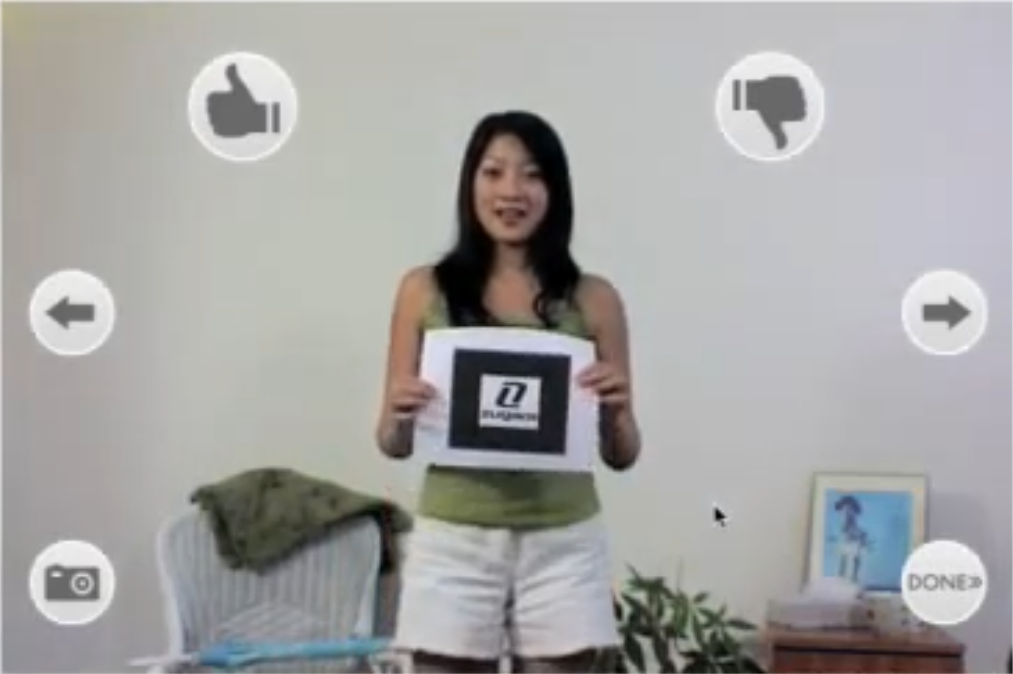
\includegraphics[scale=0.1]{marker.png} 
	}
	\subfigure[Clothing position, rotation and scale are adjusted] {
	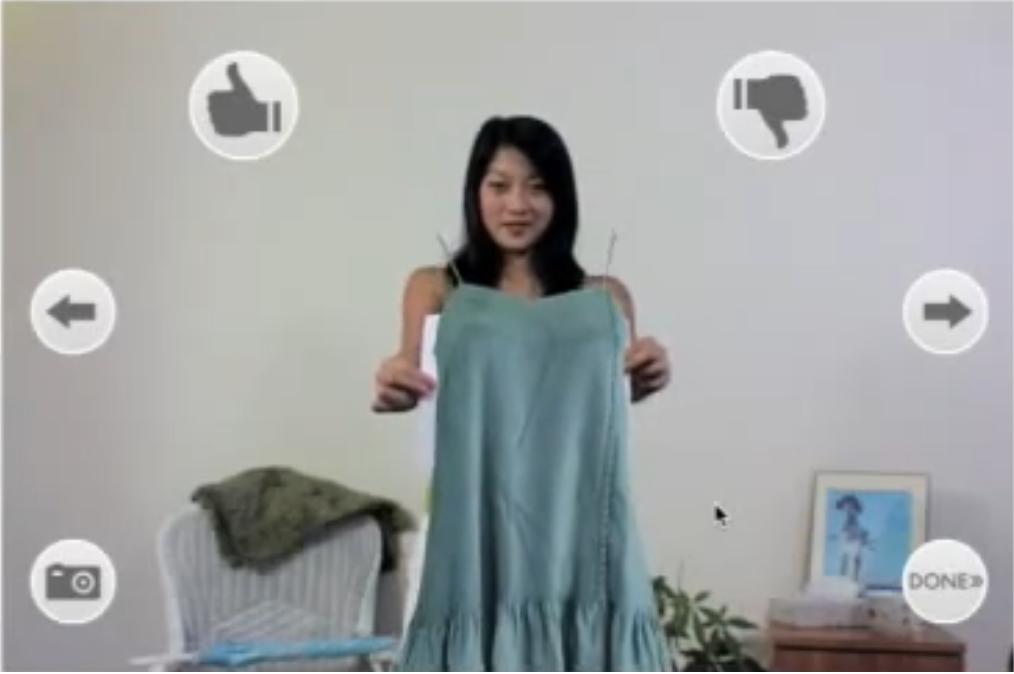
\includegraphics[scale=0.1]{marker_wrong.png} 
	}
	\subfigure[Right alignment is found] {
	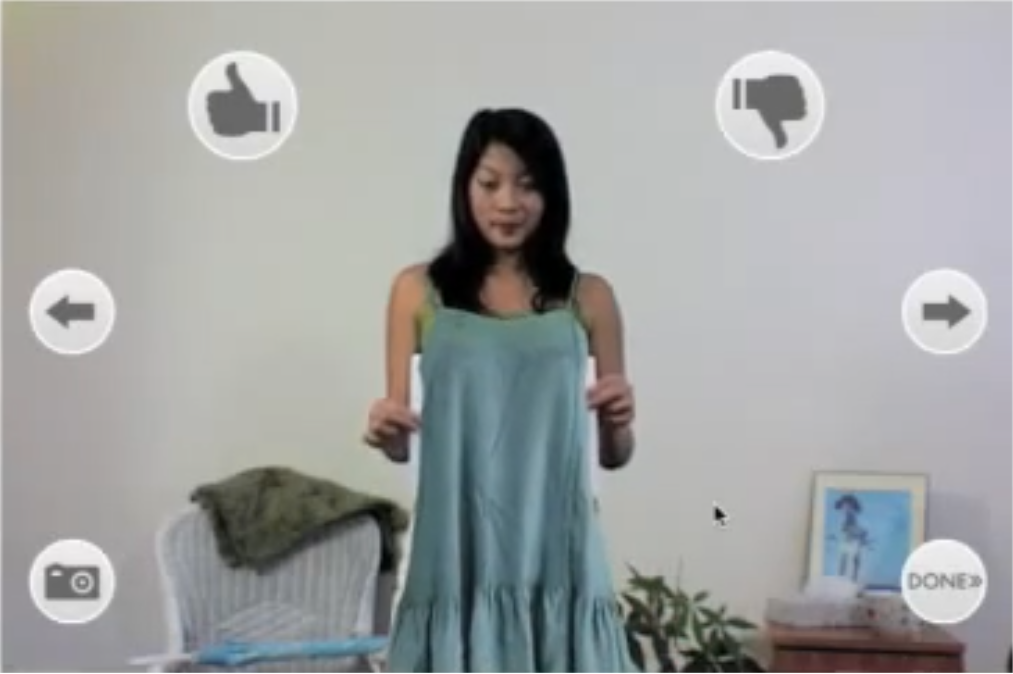
\includegraphics[scale=0.1]{marker_right.png} 
	}
\end{figure}

The introduction of the Kinect gave relatively easy and cheap access to a depth camera. And with provided middelware such as the OpenNI framework the user's pose is trackable in a quite accurate way. FaceCake\footnote{\url{http://www.facecake.com/}} \footnote{Demo: \url{http://www.youtube.com/watch?v=A0DB26zYq4A}} implemented a virtual dressing room using the Kinect and aligns the image of the clothing with the user's body using the pose tracking. This solution is currently the state of the art dressing room.

\begin{figure}[htp]
\centering
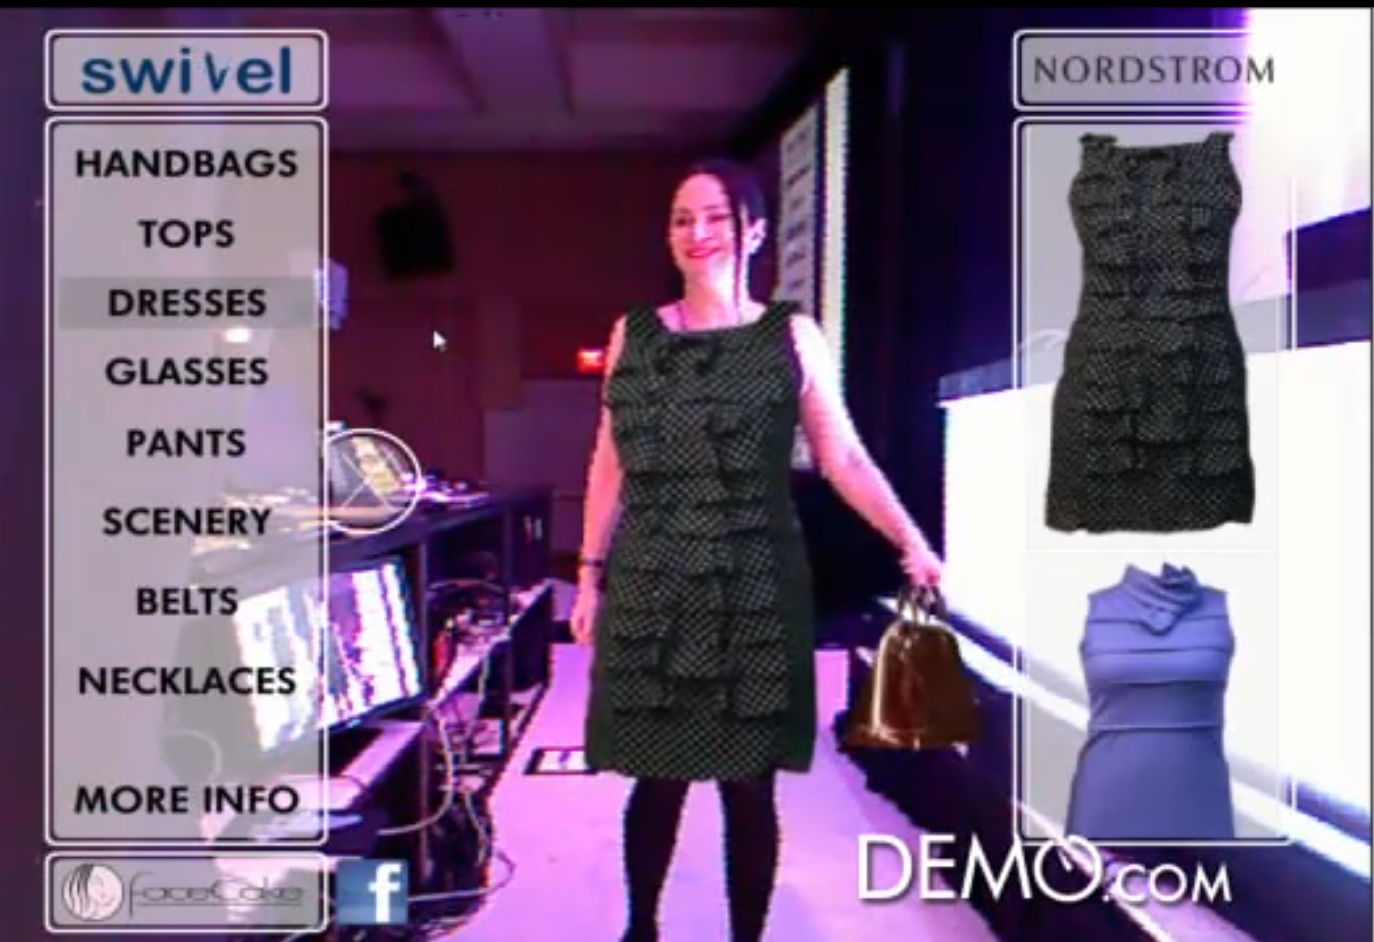
\includegraphics[scale=0.1]{facecake.png} 
\caption{Demonstration of the FaceCake virtual dressing room}
\label{fig:facecake}
\end{figure}

\subsection{Realism of clothing}

The goal of a virtual dressing room is to give a realistic visual experience of trying on clothes. Beside the alignment of the clothing, the realism is an important aspect in providing this experience. In the first versions the clothes were just static 2D images. It was only possible to see how the clothes looked from the front. In later dressing rooms such as the one created by FaceCake multiple 2D images of the clothing from different angles provided a more realistic experience, as it was possible to turn around and have a look from different sides. The clothing is still static and there is completely no interaction with the clothes besides changing location, rotation and scale.

In our approach a great improvement over the state of the art virtual dressing rooms could be made on both dimensions. In the first place the Kinect with the pose tracking gives a full skeleton of the user. Although they might be harder to track, we think that a full dressing room experience should have the option to try on pants and longsleeves too. And as our approach makes an avatar of the user and puts that avatar clothes on, it is possible to use 3D models of the clothing. Also the interaction possibly could be more realistic; the 3D modeled clothing with physics folds like real clothing and the user's avatar can have full interaction with the clothing.
In the FaceCake dressing room the clothing is always in front of the user. A more realistic experience should show the arm before the clothing, when the user's arm is before his body.

\section{Implementation}
\label{sec:implementation}

During this project we have created an augmented reality application in which the user can try on virtual clothes. We use the Kinect sensor for pose tracking, which is described in section \ref{sec:user_tracking}. For rendering the clothes in the user's environment we use the Unity game engine\footnote{\url{http://unity3d.com/}}. The virtual clothes and the way we render them is described in section \ref{sec:virtual_clothes}.

\subsection{User tracking}
\label{sec:user_tracking}

The Kinect sensor is equipped with a RGB and depth camera. The user tracking included in the OpenNI framework \footnote{\url{http://www.openni.org/}} uses the depth camera information to find one or more users. When the user stands in the calibration pose the user tracker finds the user's simplified skeleton as is given in \ref{fig:skeleton}. The 3D positions of the joints are returned along with their rotation. With this information the skeleton for the 3D avatar in Unity is known. But for the alignment of the clothing with the user's body the skeleton alone is not sufficient. The exact sizes of each bodypart should be approximated.

 \begin{figure}[htp]
\centering
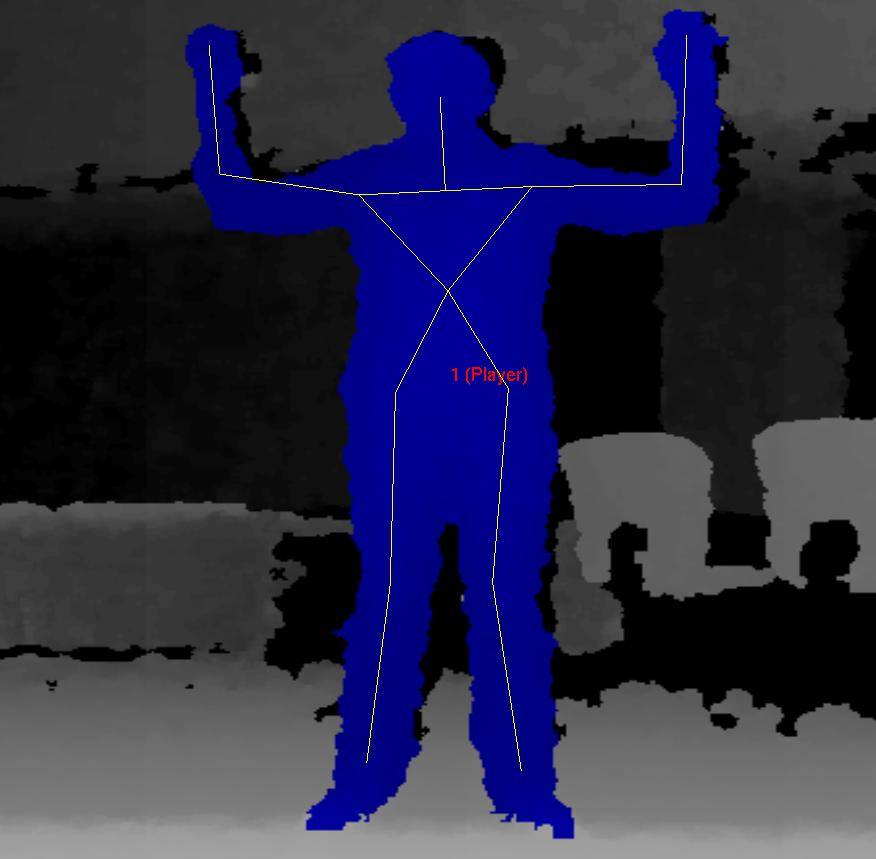
\includegraphics[scale=0.2]{usertracker.png} 
\caption{The skeleton as tracked by the OpenNI user tracker}
\label{fig:skeleton}
\end{figure}

\subsection{Size estimation}
\label{sec:size_estimation}
On calibrating the user size and length is measured. This information is used to change the user model to fit to the user body. Another feature is to recommend the right size of clothing. The length of each limb is taken by computing the distance between each joint from the skeleton.
The size of the body is taken by estimating the girth of the chest on a number of points.
\begin{figure}[htp]
\centering
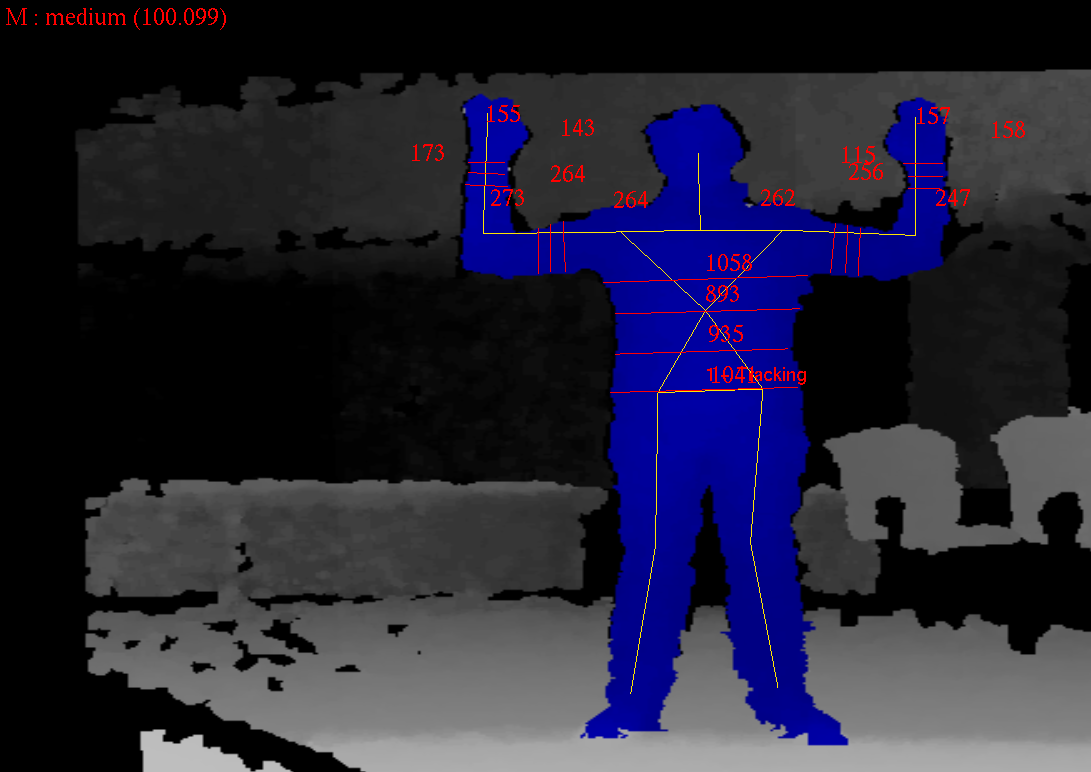
\includegraphics[scale=0.3]{size_estimation.png} 
\caption{size estimation of a user, red lines represent the places where the girth is measured. The numbers are the estimated girth of those lines.}
\label{fig:size_estimation}
\end{figure}
The girth can be measured by two methods:
\begin{itemize}
\item Computing the distance between each point on the line
\item Taking 3 points (outer left, centre and outer right) and compute the distance between those
\end{itemize}
Although the first solution seems the best, it is not robust to a noisy sensor and cloth folding. Even the slightest fold will drastically increase the users estimated girth.
The second option, although no ideal, proved more accurate than the first method.
\\
Because we can only see the front part of the user body, we have to estimate the full girth. This is done by multiplying the front part with a factor 2.1.
Before giving the estimate size of the user, we take the average over 20 frames before drawing an conclusion.


\subsection{Virtual clothes}
\label{sec:virtual_clothes}
With the 3D avatar of the user the next step in our implementation is to dress this avatar. 3D Meshes of clothing are made in Blender and imported in Unity. Unity provides 2 different clothing components that can be added to a mesh: interactive cloth and skinned cloth. Both components have features such as stretch, damping and thickness to give a real clothing experience.

\subsubsection{Interactive cloth}
\label{sec:interactive_cloth}	
Since the release of Unity 3.0 the interactive cloth is included as alternative for skinned cloth. This component turns every possible mesh into a cloth and interacts with colliders. By making the bodyparts of the user's avatar colliders, an interactive clothing should be interacting just like in reality. Interactive cloth seemed therefore a very good and realistic option for our virtual dressing room. The full interaction with environment and user body has a downside though: it is computationally complex. Besides that we experienced an incorrectly big response of the interactive cloth to the user body, resulting in catapulted clothing. These cons could be caused by the short time interactive cloth exist. If the last con is corrected, we think interactive cloth is more realistic than skinned cloth. For now however it is not useful in our implementation.
	 	
\subsubsection{Skinned cloth}
\label{sec:skinned_cloth}	 	
Skinned cloth operates very different. This component works in combination with a skinned mesh. A skinned mesh is used for characters in Unity. The character is given a bone structure and the movement of each bone affects a part of the vertices in the skinned mesh. The skinned cloth component applies clothing simulation to the vertices of the skinned mesh. Per vertex a coefficient defines how free the simulated cloth can move. The fact that this cloth component is based on a bone structure makes it very suitable for our virtual dressing room, as the user tracker supplies a skeleton of the user. Drawback is the absence of further interaction with the user and environment. The skinned cloth does not interact with colliders. This makes skinned cloth on the other hand computational simple in comparison with interactive cloth. Skinned cloth is selected for clothing simulation eventually, as it was more reliable at the moment.

\subsection{Light conditions}
\label{sec:light_conditions}
To create of more realistic scene we measure the light conditions of the RGB image. This is done by converting the image to an HSV image and take an average of the intensity from the user.
A point light in Unity will try to recreate the right light conditions.

\subsection{Body part masking}
\label{sec:bodypart_masking}
In section \ref{sec:related_work} is mentioned that the state of the art virtual dressing room by FaceCake does not provide a solution for body parts that should appear before the clothing. In our implementation the 3D information for the avatar and the clothing is available to make this more realistic. Unity gives a solution by depth masking shaders. For the body parts a material with masking shaders is selected and the clothing gets a material that is masked when behind the body parts. And as the clothing is displayed before the RGB image, the body part is shown as if it is before the clothing (Figure \ref{fig:shader}).

 \begin{figure}[htp]
\centering
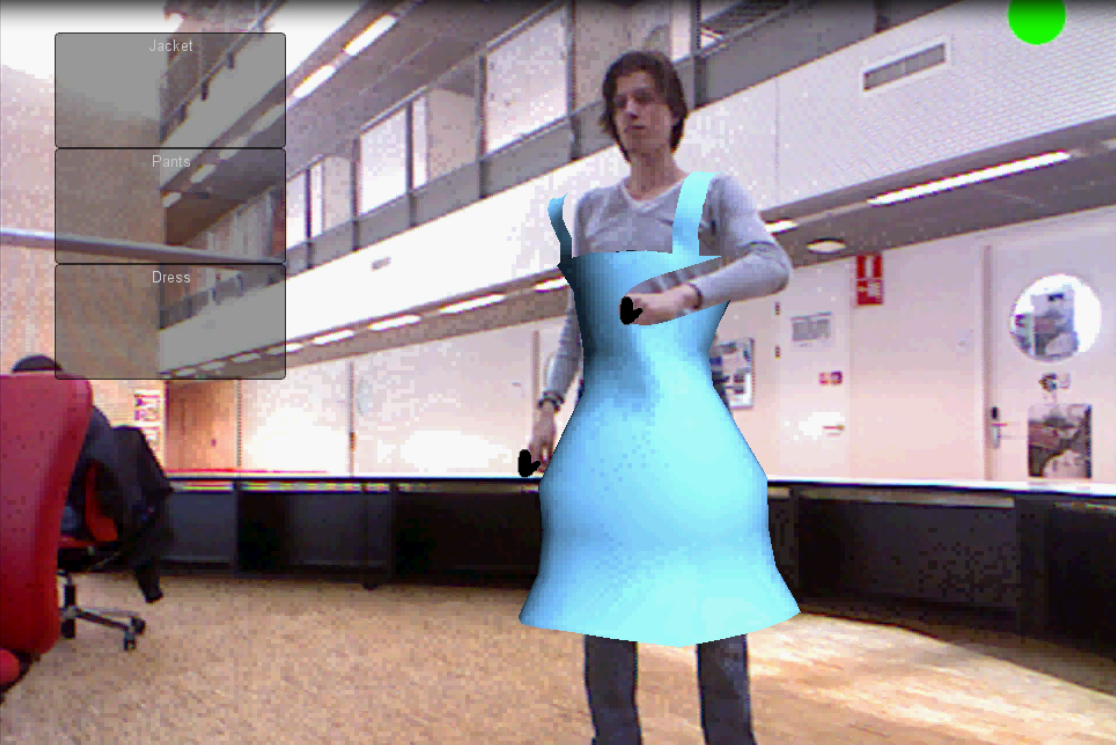
\includegraphics[scale=0.3]{show_shader_morris.png} 
\caption{The body part maskes the clothing and shows the background image}
\label{fig:shader}
\end{figure}


\subsection{Application overview}
\label{sec:application_overview}
The GUI of the virtual dressing room consists of an RGB image, 3 buttons and a calibration progress marker. To use the application the user first has to calibrate with the system. This is done by taking the calibration pose (Figure ~\ref{fig:calibrationPose}), it will take a few secondes before the system is calibrated. The marker on the top right of the screen will display the calibration progress (Figure ~\ref{fig:progressmarker}).
\begin{figure}[h!]
\centering
	\subfigure[looking for user] {
	
\includegraphics[scale=0.5]{lookingforuser.png} 
	}
	\subfigure[looking for calibration pose] {
	
\includegraphics[scale=0.5]{looking.png} 
	}
	\subfigure[calibrating] {
	
\includegraphics[scale=0.5]{calibrating.png} 
	}
	\subfigure[calibrated] {
	
\includegraphics[scale=0.5]{calibrated.png} 
	}
	\caption{Different progress marker states} 
	\label{fig:progressmarker}
\end{figure}

\begin{figure}
\centering
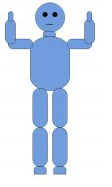
\includegraphics[scale=0.5]{calibrationPose.png} 
\caption{calibration pose for kinect}
\label{fig:calibrationPose}
\end{figure}

When the calibration step is completed the user can change their clothing by activating or deactivating the available buttons on the screen. This can be done by hovering either the left or right hand over the button.
Items currently available in this project:
\begin{itemize}
\item Jacket.
\item Pants 
\item Dress.
\end{itemize}
Here a few examples of users wearing the virtual clothes.
\begin{figure}[h!]
\centering
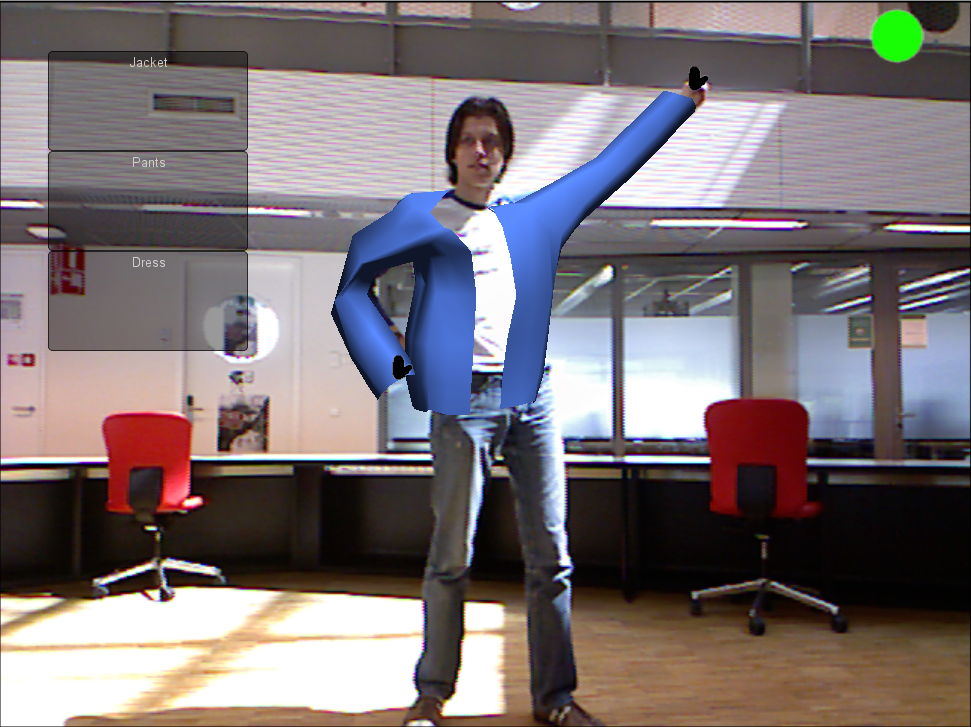
\includegraphics[scale=0.4]{GUI_jacket_morris.png} 
\caption{A user wearing a blue jacket.}
\label{fig:jacket_morris}
\end{figure}

\begin{figure}[h!]
\centering
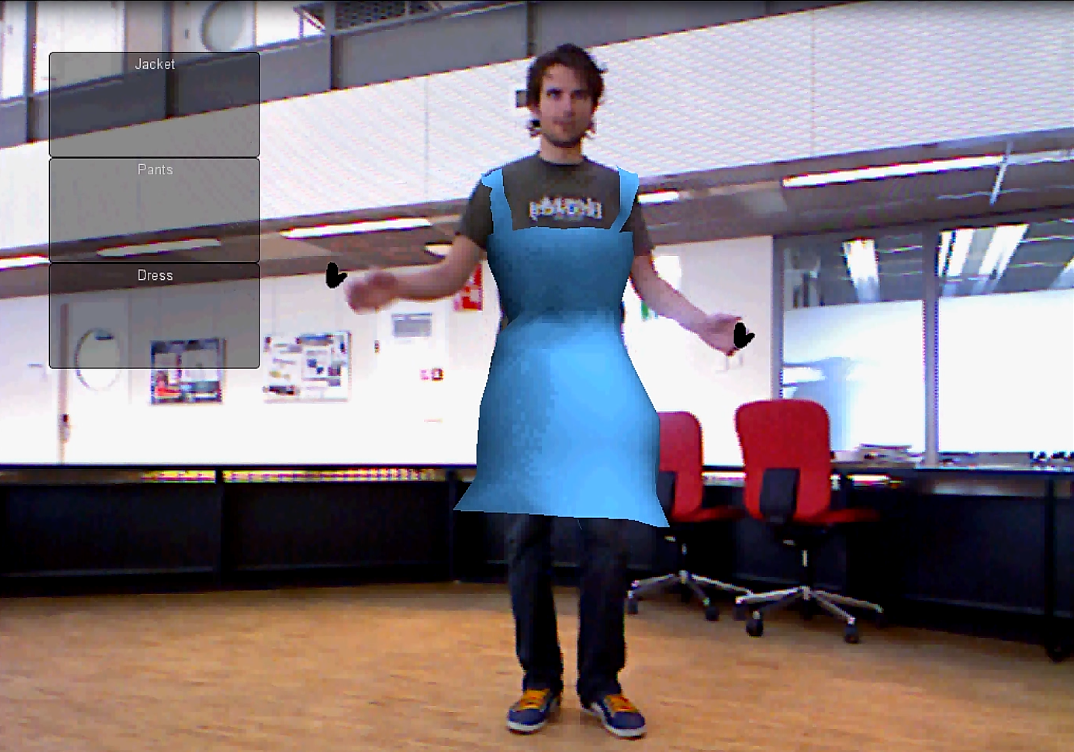
\includegraphics[scale=0.4]{dress_fedde.png} 
\caption{A user wearing a dress.}
\label{fig:dress_fedde}
\end{figure}

\section{Discussion}
\label{sec:discussion}

The implementation discussed in section \ref{sec:implementation} has several limitations which we will discuss in this section, along with suggestions for removing these limitations. 

For any augmented reality application it is important to have realistic interaction between the user and virtual objects, in this case the virtual clothing. Interaction with the clothing comes in two forms, firstly having the cloth move with the user as if he/she is wearing them, and secondly direct physical interaction between the clothing and the user body. These two forms of interaction correspond to the two types of clothing simulation described in section \ref{sec:virtual_clothes}: skinning the cloth to the user skeleton allows for realistic movement, while the interactive cloth includes a physics simulation that allows for correct interaction between the cloth and physical objects in the scene, such as the user body. A combination between the two approaches could combine the best attributes of both. Such an approach would be to add collision detection to the vertices in the clothing mesh, but restricting the resulting transformation to the volume defined by the skinned cloth coefficients.

Our approach to display the RGB image captured by the sensor as a background image and masking out parts of the clothing by checking for occlusion by the user avatar also has some limitations. First, because the mesh of the user avatar is constructed from primitive shapes it does not correspond exactly to the user's shape and thus the masked image includes parts of the body which should not be displayed and clips off parts which should be. Secondly, since other objects from the user's environment have no mesh representation they are not used in this masking process and can not occlude the clothing. As a result the clothing might be projected over an object which occludes the user and should thus occlude the clothing. The Kinect sensor outputs the color and depth of each pixel, thus a simple solution would be to display the image not as a background image but by using a pixel shader which writes each pixel's color value into the depth buffer and should thus occlude parts of the virtual objects which are behind it in the depth buffer.

Evaluatie van size estimation moet grotere dataset hebben

Kleding zou meer realistisch zijn met hulp van 3d artists (textures, pasvorm)

\section{Conclusion}
\label{sec:conclusion}

This report has presented an augmented reality application in which users can select and try on virtual clothes. These clothes are rendered on a screen over the image of the user and the lighting of the rendered clothing is adapted to match the light intensity of the user's environment. The main features of this application, corresponding to the goals in section \ref{sec:project_goals}, are as follows:
\begin{itemize}
\item The clothing is correctly aligned with the user's position and movement by skinning the clothing models to a skeleton rig which is controlled by the Kinect sensor's skeleton tracking.
\item The clothing moves and folds realistically by applying Unity's clothing simulation to the clothing models.
\item The clothing is realistically rendered by adapting the light intensity in the virtual scene to match the user's environment and by masking out the parts of the rendered clothing which would be occluded by the user.
\end{itemize}

The presented application is an improvement over similar existing augmented reality applications in that it offers both full user pose tracking using the Kinect, as well as 3-dimensional clothing models with cloth physics simulation such that it can be viewed from any angle, smoothly moves and rotates with the user, and reacts similar to real clothing.

As a technology demo, the presented application shows how accurate augmented reality interaction with virtual objects can be realized using a depth camera with pose tracking. Considering that such sensors are now being released as consumer products we expect much future work in augmented reality will take advantage of these technologies.

Although the size estimation does work well under a simple algorithm, it will be much harder to estimate the true girth. not knowing what clothing the user is wearing, and how much distance there is between the clothes and the user body (sloppy vs. tight clothing). And because the kinect can only see the front side of the body, it has to estimate the back. 
Accuracy might increase by using a large dataset of trainings data and a linear regressing classifier to estimate the girth.

\end{document}
